\subsection{SP-9 (KAB)}
Asymetrické kryptosystémy (šifra RSA, Diffie-Hellman, RSA digitální podpis), hešovací funkce (SHA-2, HMAC). Digitální podpis. Certifikáty, certifikační autority.

\subsubsection*{Asymetrické šifry}
\begin{itemize}
	\item pro šifrování a dešifrování se používají různé klíče
	\item pomocí privátního klíče šifrujeme, promocí veřejného klíče dešifrujeme
	\item privátní klíč nelze odvodit z veřejného klíče v rozumném čase
	\item každý subjekt má svůj vlastní pár veřejný-privátní klíč
\end{itemize}
\textbf{princip RSA}
\begin{itemize}
	\item šifrovací systém založený na modulárním umocňování
	\item dvojice ($e, n$) je veřejný klíč ($e$ --- veřejný exponent, $n$ --- modul)
	\item $n$ je součinem dvou velkých prvočísel $p$ a $q$, tedy $n = pq$ a gcd($e, \varphi(n)$) = 1
	\item zašifrováni plaintextu --- písmena se převedou na numerické ekvivalenty, vytvoří se bloky s největší možnou velikostí --- $E(m) = c = |m^e|_n$, $0 < c < n$ ($m$ je vytvořený blok plaintextu, $c$ je výsledný blok ciphertextu)
	\item k dešifrování je nutná znalost inverze $d$ čísla $e$ modulo $\varphi(n)$ --- gcd($e, \varphi(n)$) = 1, inverze tedy existuje --- $D(c) = |c^d|_n = |m^{ed}|_n$, $e$ a $d$ jsou inverzní modulo $\varphi(n)$, tedy $ed \equiv 1$ (mod $\varphi(n)$), tedy $ed = 1 + k \cdot \varphi(n)$, z toho $\Rightarrow |m^{ed}|_n = |m^{1 + k \cdot \varphi(n)}|_n = |m \cdot (m^{\varphi(n)})^{k}|_n$, a dle Eulerovy věty $m^{\varphi(n)} \equiv 1$ (mod $n$), tedy celkově $D(c) = |m|_n$
	
	\item dvojice ($d, n$) tvoří soukromý klíč 
	
	\item existuje možnost, že $m$ a $n$ jsou soudělné, ale je extrémně malá
\end{itemize}

\textbf{Generování RSA klíčů}
\begin{itemize}
	\item jak hledat $p$ a $q$?
	\item subjekt nalezne 2 velká náhodná čísla $p$ a $q$ s 340 dekadickými číslicemi
	\item z věty o prvočíslech plyne, že pravděpodobnost toho, že takto vybraná čísla jsou prvočísla, je cca $2 /$ log($10^340$)
	\item pro nalezení prvočísla je potřeba v průměru 1 / ($2 /$ log($10^340$)) $\approx$ 400 testů takových čísel
	\item exponent $e$ by následně měl být zvolen jako číslo větší než $p$ a $q$ --- $2^e$ by mělo být větší než $n$, aby šifrování i dešifrování muselo používat redukci modulo $n$ a nešlo pouze odmocnit
\end{itemize}

\textbf{Bezpečnost RSA}
\begin{itemize}
	\item modulární umocňování potřebné k šifrování zprávy s použitím RSA může být provedeno při velikosti modulu a bloku cca 680 dekadických číslic v řádech milisekund
	\item dešifrovací exponent $d$ nelze z dvojice ($e, n$) snadno odvodit, protože je potřeba znát hodnota $\varphi(n)$ --- pro rychlé spočítání je třeba znát faktorizaci $n = pq$
	\item i v případě cca 100-číslicových $p$ a $q$ (tedy 200-číslicového modulu $n$) trvá nejrychlejším známým algoritmům faktorizace kolem 250 let
	\item náročnost prolomení je tím větší, čím větší je modul 
	\item ochrana proti speciálním rychlým technikám faktorizace $n$: např. obě hodnoty $p-1$ a $q-1$ by měly mít velký prvočíselný faktor, tedy malé gcd($p-1, q-1$) a rozdíl $p - q$ by měl být dostatečně velký
\end{itemize}

\textbf{Digitální podpis s použitím RSA}
\begin{itemize}
	\item uvažujme 2 subjekty, každý má svůj pár privátní-veřejný klíč ($PK_1, VK_1$), ($PK_2, VK_2$)
	\item subjekt 1 chce poslat podepsanou zprávu
	\item subjekt 1 ji podepíše: $S = D_{PK_1}(m) = |m^{d_1}|_{n_1}$
	\item subjekt 1 zašifruje pro subjekt 2: $c = E_{VK_2}(S) = |S^{e_2}|_{n_2}$ (pokud $n_2 > n_1$, jinak je nutné rozdělit $S$ do bloků o velikosti menší než $n_2$ před šifrováním)
	\item subjekt 2 nejprve dešifruje svým privátním klíčem, následně použije šifrovací transformaci veřejným klíčem subjektu 1 pro odkrytí původního obsahu
	\item subjekt 2 si je tedy jistý, že zpráva přišla od subjektu 1, a zároveň subjekt 1 nemůže popřít, že danou zprávu poslal
\end{itemize}

\textbf{Urychlení RSA výpočtů}
\begin{itemize}
	\item urychlení šifrování --- doporučená množina exponentů $e$ s nízkou Hammingovou váhou
	\item urychlení dešifrování --- použití Čínské věty o zbytcích (RSA-CRT) (rozklad čísel, počítá se s čísly poloviční délky)
\end{itemize}

\textbf{Diffie-Hellmann}
\begin{itemize}
	\item algoritmus pro ustanovení společného klíče
	\item subjekt A a B si veřejně dohodnou prvočíslo $m$ a bázi $a$ ($1 < a < m$), přesněji grupu řádu $m-1$
	\item subjekt A si náhodně zvolí číslo $k_A$ takové, že $0 < k_A < m$ a gcd($k_A, m - 1$) = 1, spočítá $y_a = |a^{k_A}|_m$ a odešle ho B
	\item subjekt B si náhodně zvolí $k_B$ takové, že $0 < k_n < m$ a gcd($k_B, m - 1$) = 1, spočítá $y_B = |a^{k_B}|_m$ a odešle ho A
	\item A i B spočítají sdílený klíč $K = |{y_B}^{k_A}|_m = |(a^{k_B})^{k_A}|_m = |a^{k_A \cdot k_B}|_m = |(a^{k_A})^{k_B}|_m = |{y_A}^{k_B}|_m$
	\item útočník nemůže z $|a^{k_A}|_m$ ani z $|a^{k_B}|_m$ spočítat $K = |a^{k_A \cdot k_B}|_m$ --- tzv. Diffie-Hellmanův problém, DHP
	\item není složitější než DLP (problém diskrétního logaritmu), a zdá se že ale není ani jednodušší

\end{itemize}

\textbf{El Gamal}
\begin{itemize}
	\item vzniká úpravou Diffie-Hellman
	\item A zvolí číslo $g$ a prvočíslo $m$, $1 < g < m$, a $g$ je generátor odpovídající grupy řádu $m - 1$
	\item A si náhodně zvolí soukromý klíč $k_A$ tak, že $0 < k_A < m$, spočítá $y_A = |g^{k_A}|_m$
	\item A zveřejní uspořádanou trojici ($m, q, y_A$) jako veřejný klíč, $k_A$ je soukromým klíčem
	\item B chce odeslat A zprávu $p$
	\item B si náhodně zvolí číslo $k_B$ ($0 < k_B < m$), spočítá $y_B = |g^k_B|_m$
	\item B spočítá sdílený klíč $K = |{y_A}^{k_B}|_m = |g^{k_A \cdot k_B}|_m$ 
	\item B zašifruje zprávu $p$ pomocí vztahu $c = |p \cdot K|_m$
	\item B odešle A uspořádanou dvojici ($y_B, c$)
	\item A si spočítá $K = |{y_B}^{k_A}|_m = |g^{k_A \cdot k_B}|_m$
	\item A si spočítá $|k^{-1}|_m$ (přes REA)
	\item A dešifruje zprávu: $p = |c \cdot K^{-1}|_m = |p \cdot K \cdot K^{-1}|_m = |p|_m$
\end{itemize}

\subsubsection*{Hash funkce}
\begin{itemize}
	\item základní pojmy: jednosměrnost, bezkoliznost
	\item \textbf{Jednosměrnost:} $f: X \rightarrow Y$, je snadné z jakékoliv hodnoty $x \in X$ vypočítat $y = $ f($x$), ale je výpočetně nemožné pro náhodný obraz $y \in $f($X$) najít vzor $x \in X$, aby $y = $ f($x$)
	\item \textbf{Hashovací funkce} je jednosměrná (1. typu --- neexistují zadní vrátka pro zpětný výpočet) a bezkolizní, zároveň pro různé vstupy vrací stejně dlouhý výstup (hash)
	\item \textbf{Orákulum:} libovolná stroj, který na základě vstupu odpoví nějakým výstupem, na stejný vstup odpovídá stejným výstupem
	\item \textbf{Náhodné orákulum:} na nový vstup odpovídá náhodným výběrem z množiny vstupů
	\item Hashovací funkce se má chovat jako náhodné orákulum (bezpečnostní vlastnosti)
	\item \textbf{Bezkoliznost 1. řádu:} Hash fce $h$ je odolná proti kolizím 1. řádu, jestliže je výpočetně nezvládnutelné nalezení libovolných dvou různých (byť nesmyslných) zpráv $M$ a $M'$ tak, že $h(M) = h(M')$
	\item bezkoliznost se využívá k digitálním podpisům
	\item nepodepisuje se zpráva (moc dlouhá) ale její hash
	\item bezkoliznost zaručuje, že je složité nalézt 2 dokumenty se stejným hashem --- proto lze podepisovat hash
	\item \textbf{Bezkoliznost 2. řádu:} Hash funkce $h$ je odolná proti kolizi 2. řádu, jestliže pro jakýkoliv vzor $x$ je výpočetně nezvládnutelné nalézt 2. vzor $y \neq x$ tak, že  $h(x) = h(y)$
	\item \textbf{Odolnost pro nalezení kolize 1. řádu:} pokud se hash funkce s hashem délky $n$ bude chovat jako náhodné orákulum, složitost nalezení kolize s 50 \% pravděpodobností je $\approx 2^{n \over 2}$ (narozeninový paradox)
	\item \textbf{Odolnost proti nalezení kolize 2. řádu:} pokud se hash funkce s hashem délky $n$ bude chovat jako náhodné orákulum, složitost nalezení 2. vzoru je $\approx 2^{n}$
	\item pokud pro konkrétní hash funkci lze nalézat vzory/kolize rycheji, hovoříme o prolomení hashovací funkce
	\item při hashování se typicky zpráva rozdělí na bloky, poslední blok se doplní (např. jednou 1 a pak samé 0, aby otisky zpráv co by na konci měly např. jen víc nul byly jiné)
	\item pro konkrétní bloky se využívá kompresní funkce $f$, která z předchozího kontextu $H_{i-1}$ a bloku $M_i$ vytvoří kontext $H_i$
	\item při konstrukci hash funkce dle následujícího obrázku bezkoliznost kompresní funkce zaručuje bezkoliznost celé hashovací funkce
\end{itemize}

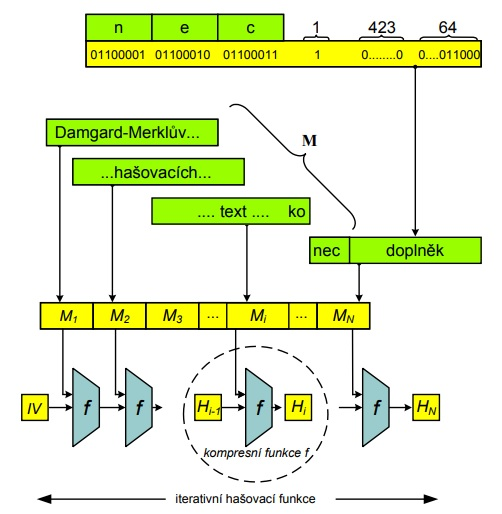
\includegraphics[width=0.55\textwidth]{img/SP-9_0.jpg}

\begin{itemize}
	\item jako kompresní funkce se typicky používá bloková šifra --- kontext $H_{i-1}$ je vstup, blok $M_i$ je klíč
	\item dle Davies-Meyerovy konstrukce se ještě po zašifrování přičte (XOR) původní kontext
\end{itemize}

\textbf{HMAC}
\begin{itemize}
	\item nepadělatelný integritní kód zprávy
	\item pro zprávu se spočítá za použití tajného klíče $K$
	\item detekuje chyby při přenosu, zabraňuje neoprávněné změně zprávy
	
	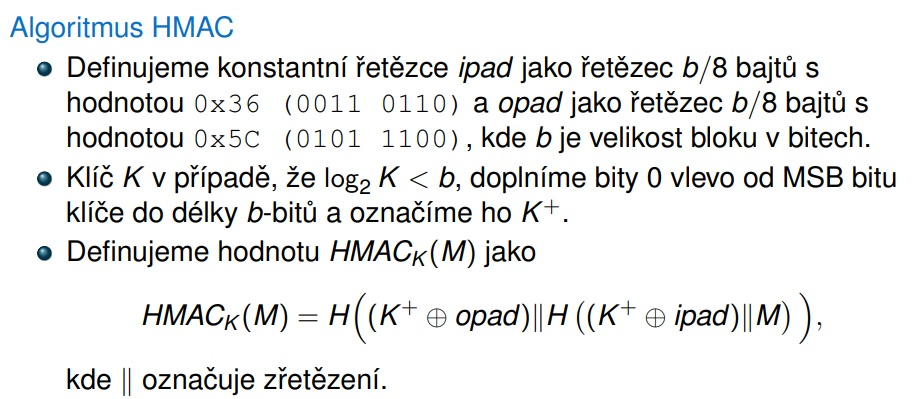
\includegraphics[width=0.7\textwidth]{img/SP-9_1.jpg}
\end{itemize}

\subsubsection*{Public Key Infrastructure}
\begin{itemize}
	\item jak distribuovat tajné symetrické klíče? distribuujeme veřejné klíče, následně si tajné klíče předáme za použití asymetrického šifrování
	\item jak distribuovat veřejné klíče? jak zabránit možnosti podvrhnutí?
	\item \textbf{Zveřejnění veřejných klíčů}
	\begin{itemize}
		\item zasílání veřejných klíčů přímo
		\item rychlé a jednoduché
		\item není odolné proti podvržení
	\end{itemize}
	\item \textbf{Veřejně dostupný adresář}
	\begin{itemize}
		\item vyšší úroveň bezpečnosti
		\item distribuci zajišťuje důvěryhodná autorita/správce
	\end{itemize}
	
	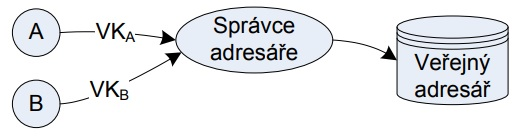
\includegraphics[width=0.4\textwidth]{img/SP-9_2.jpg}
	
	\item \textbf{Autorita pro veřejné klíče}
	\begin{itemize}
		\item přísnější dohled na distribuci veřejného klíče z adresáře
		\item autorita má svůj pár veřejný-privátní klíč, každý účastník musí znát její veřejný klíč
	\end{itemize}
	
	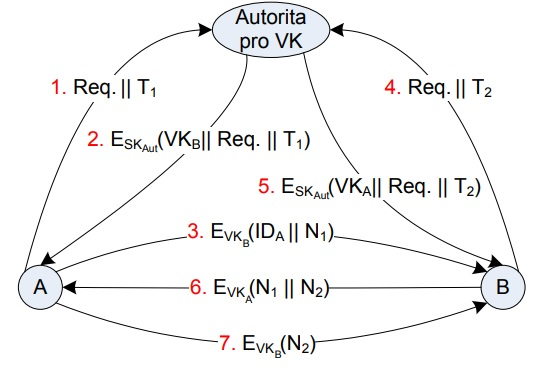
\includegraphics[width=0.45\textwidth]{img/SP-9_3.jpg}
	
	\item \textbf{Certifikace veřejných klíčů}
	\begin{itemize}
		\item distribuce veřejného klíče bez kontaktu se třetí stranou
		\item Certifikát: struktura obsahující veřejný klíč držitele, identifikační údaje držitele, dobu platnosti, další údaje vytvořené CA a zejména podpis CA
		\item Certifikační Autorita (CA): důvěryhodná třeí strana, která na základě žádosti vydává a aktualizuje certifikáty --- certifikáty vytvořené CA lze ověřit jejím veřejným klíčem	
	\end{itemize}
	
	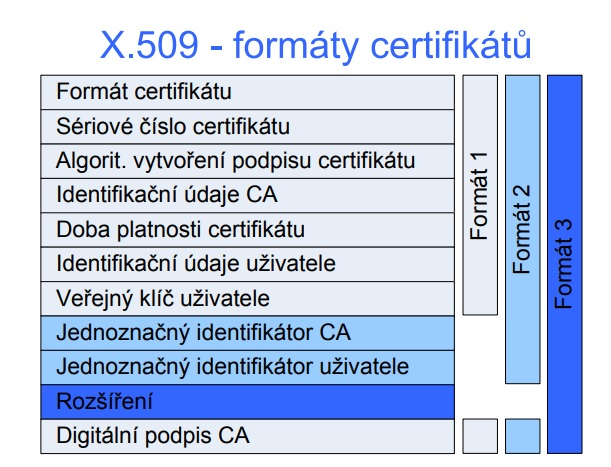
\includegraphics[width=0.5\textwidth]{img/SP-9_4.jpg}
	
	\item certifikáty mohou být podepsané ve stromové struktuře --- certifikát držitele podepsaný CA$_1$, její certifikát podepsaný CA$_2$...
	\item kořenové certifikáty musí být distribuovány jinak (typicky např. s operačním systémem)
\end{itemize}